\documentclass[runningheads]{llncs}
%
\usepackage{graphicx}
\usepackage{multirow}
\usepackage{subcaption}
\usepackage[center]{caption}
\usepackage{fancyhdr}
\pagestyle{fancy}

\begin{document}
\pagestyle{fancy}
\fancyhead{} % clear all header fields
\renewcommand{\headrulewidth}{0pt} % no line in header area
\fancyfoot{} % clear all footer fields
\rfoot{\thepage}           % page number in "outer" position of footer line
\footnotetext{https://github.com/itsmeabiii/-Group-G--MiniPaper} % other info in "inner" position of footer line
\footnotetext{https://github.com/laxmimerit/twitter-suicidal-intention-dataset}


\title{Analyzing Tweets and Predicting Suicide Ideation}
%
%\titlerunning{Abbreviated paper title}
% If the paper title is too long for the running head, you can set
% an abbreviated paper title here
%
\author{Castro, Karmela\inst{1}\and Davocol, Abigail\inst{1}\and
Facultad, Joever\inst{3} Ambita, Ara Abigail \inst{4} }
%

\authorrunning{F. Author et al.}
% First names are abbreviated in the running head.
% If there are more than two authors, 'et al.' is used.
%
\institute{Universtiy of the Philippines Visayas, Miagao, Iloilo, Philippines \\
\email{kfcastro1@up.edu.ph}\\ 
\email{apdavocol@up.edu.ph}\\
\email{jgfacultad@up.edu.ph}\\
\email{aeambita@up.edu.ph}\\
}

%
\maketitle              % typeset the header of the contribution
%
\begin{abstract} Suicide is one of the leading causes of death. In 2020, 3.2 million planned suicide attempts and 1.2 million attempted suicide. However, recently there is a trend wherein people tweet their suicidal intention on Twitter. In this paper, twitter suicidal dataset is fed to classification algorithms such as GaussianNB, BernoulliNB, RandomForest(n\_est = 100, n\_est = 400) and Logistic Regression. The performance metrics shows promising results wherein RandomForest n\_est=400 outranked the other classification algorithms in predicting suicide ideation. This study provides further information on what classification model is suitable to be utilized for predicting suicide ideation and provide insights on what feature models can be used in future studies to improve the performance metrics of the model.


\keywords{Twitter data  \and suicide ideation \and Naives Bayes \and RandomForest \and Logistic Regression.}
\end{abstract}
%
%
%
\section{Introduction}
Based on the data from the Centers for Disease Control and Prevention (n.d), in 2019 alone 9 person out of 100,000 died by suicide worldwide. Between the year 2000 and 2018 the suicide rate soared by 30\%, then it fell in 2019 and 2020. However, despite that decrease in the recent years suicide remains to be one of the leading cause of mortality in the United States, and accounting for 45,979 deaths by suicide in 2020 alone. This equates to approximately one death for every 11 minutes. In the same year,  an estimated 12.2 million American individuals seriously considered suicide. 3.2 million planned suicide attempts, and 1.2 million attempted suicide. 
\paragraph{}
Recently, a lot of people are posting their suicidal intentions or tendencies on various social media platforms such as Twitter. This indicates that social media sites platforms can potentially be used as a tool to help prevent suicide. Today, social media platforms are rapidly being utilized by a lot of people not only to interact and receive news or information, but also to convey signs of emotional distress and suicidal tendencies. According to Twitter data, suicidal ideation is often linked to negative feelings such as shame and despair, as well as a number of regional and ecological characteristics (Morese et al., 2022).
\paragraph{}
By being able to detect suicidal ideation through the use of data from social media platforms such as Twitter, proper care and help can immediately be done in order to check up on those individuals and give them the proper care and potentially save a life.
\paragraph{}
Therefore, the objective of this paper is to:
\begin{enumerate}
\setlength{\itemindent}{.5in}
  \item Evaluate Term Frequency-Inverse Document Frequency as a feature extraction method and evaluate its performance metrics on different classification models.
  \item Evaluate performance metrics of the Gaussian Naïve Bay, Bernoulli Naïve Bayes, Random Forest and Logistic Regression in predicting tweet with suicide ideation and no intention.
  \item Determine the classification algorithm that can best predict the tweets with suicide intention and tweets with no suicide intention.
\end{enumerate}

\subsection{Related Works}
O’Dea et al. (2015) examined the level of concern for a suicide-related Twitter posts using human coders and machine learning processes. There were three levels of concern that were used: ‘strongly concerning’, ‘possibly concerning’, and ‘safe to ignore’. ‘Strongly concerning’ level are tweets that have a convincing display of serious suicidal ideation. ‘Possibly concerning’ is the default category for all tweets. On the other hand, ‘safe to ignore’ are tweets with no reasonable evidence that the risk of suicide is present. The dataset used contained a total of 14,701 suicide-related tweets, where 14\% were coded and analyzed by human researchers. Results showed that 14\% of suicide-related tweets were classified as ‘strongly concerning’, others were ‘possibly concerning’ (56\%) and (29\%) were considered ‘safe to ignore’. In contrast, the remaining dataset was used for machine learning processes. Word frequencies and all words were used as features. They used two machine learning algorithms for text classification, Support Vector Machines (SVMs) and Logistic Regression. According to O’Dea et al. (2015), the automated classifier correctly identified 80\% of ‘strongly concerning’ tweets and achieved the same accuracy as the human coders. The study concluded that “Twitter is used by individuals to express suicidality and that such posts evoked a level of concern that warranted further investigation.” However, it is still unknown whether the "strongly concerning" tweets were genuine suicidal statements.
\paragraph{}
In a study by Sinyor et al.  (2020), the researchers identify the associations between specific social media content and suicide deaths. For the methods, multivariable logistic regression was used to examine whether tweet characteristics were associated with increases or decreases in suicide deaths in Toronto in the 7 days after posting, compared with a 7-day control window. The results shows that the elements independently associated with increased subsequent suicide counts were tweets about the suicide of a local newspaper reporter (OR = 5.27, 95\% CI = [1.27, 21.99]), 'other' social causes of suicide (e.g. cultural, relational, legal problems; OR = 2.39, 95\% CI = [1.17, 4.86]), advocacy efforts (OR = 2.34, 95\% CI = [1.48, 3.70]) and suicide death (OR = 1.52, 95\% CI = [1.07, 2.15]) while the elements most strongly independently associated with decreased subsequent suicides were tweets about murder suicides (OR = 0.02, 95\% CI = [0.002, 0.17]) and suicide in first responders (OR = 0.17, 95\% CI = [0.05, 0.52]).
\paragraph{}
These findings of the study largely comport with the theory of suicide contagion and associations observed with traditional news media. They specifically suggest that tweets describing suicide deaths and/or sensationalized news stories may be harmful while those that present suicide as undesirable, tragic and/or preventable may be helpful. These results suggest that social media is both an important exposure and potential avenue for intervention. 

\section{Methodology}
The twitter-suicidal\_data.csv file is a dataset created by Laxmi Kant and was obtained from “twitter-suicidal-intention-dataset” repository at GitHub. The dataset has 9119 observations. It contains the tweet data of suicidal intention and no intention data [2]. As seen in Figure 1, tweet is the text data and intention is the target label [2]. The tweets’ intention were classified into two category, 1 (suicidal) and 0 (non-sucidal). The suicidal tweet contains messages about anxiety, depression, hopelessness, wanting to die, suicide attempt or any other tweets related to suicidal thoughts or suicidal ideation. The non-suicidal tweet contains messages that is not relevant or related to suicide.
\begin{figure}
    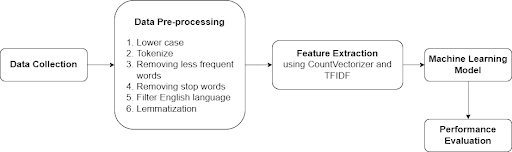
\includegraphics[width=\textwidth]{framework.png}
    \caption{Framework of the study.} \label{fig1}
\end{figure}

\subsection{Data Collection}
The twitter-suicidal\_data.csv file is a dataset created by Laxmi Kant and was obtained from “twitter-suicidal-intention-dataset” repository at GitHub. The dataset has 9119 raw observations. It contains the tweet data of suicidal intention and no intention data [2]. As seen in Figure 1, tweet is the text data and intention is the target label [2]. The tweets’ intention were classified into two category, 1 (suicidal) and 0 (non-sucidal). The suicidal tweet contains messages about anxiety, depression, hopelessness, wanting to die, suicide attempt or any other tweets related to suicidal thoughts or suicidal ideation. The non-suicidal tweet contains some hate messages and expression of negative feelings however they don’t express suicide ideation.

\indent As observed in figure 2 below, there are 5121 tweets without suicide intentions and 3998 tweets that have suicide intention. This indicates that the tweets without suicide intentions is greater than the tweets with suicide intentions.

\begin{figure}
    \centering
    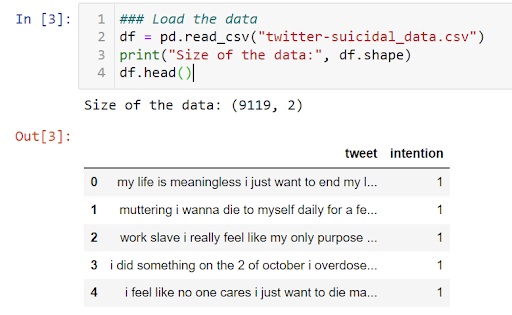
\includegraphics[width=8cm]{datacol.png}
    \caption{The raw twitter-suicidal\_data dataset.} \label{fig1}
    \vspace{1cm}
    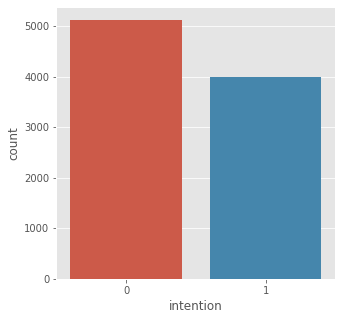
\includegraphics[width=8cm]{intentiongraph.png}
    \caption{No. of tweets with suicide intention (1) vs. No. of tweets without suicide intention (0).} \label{fig1}
\end{figure}

\subsection{Data Pre-processing}
Data pre-processing is a step to transform raw data into a format that can be understood by the computer and machine learning models. The following are the steps performed to prepare the data for training and testing with the model.

\textbf{Lower case}. The texts are converted into lower case text. For example, the word “Life” would be “life” after converting.This is to have a consistent format text throughout the data.

\textbf{Tokenize}. The sentences in every data are converted to words.

\textbf{Removing less frequent words}. Less frequent words are removed as they are rarely used and also to remove noise in the data.

\textbf{Removing stop words}. NTLK’s English stop word corpus was used to remove English stop words in the tweets, such as “a”, “an”, “of”, “the”, etc.

\textbf{Filter English language}. The non-English words were removed from the data so that only English words remain.

\textbf{Lemmatization}. Textblob library was used to apply a morphological analysis to words (Geekforgeeks, 2022). For example, the lemma or dictionary form of the word “meeting” is “meet” and for “was” is “be” (Geekforgeeks, 2022).

\subsection{Feature Extraction}
This study used Count Vecotorizer and TFIDFTransformer to extract the feature from the dataset wherein the TFIDFTransformer normalizes the data after it has been tokenized and counted by Count Vectorizer (Geek Culture, 2021). We used the TF-IDF as an feature extraction method because the TF-IDF highlights the relevance of the term in understanding the document or dataset. This is due to the fact that TF-IDF is composed of two components: Term Frequency (TF) and Inverse Document Frequency (IDF). The term frequency denotes the frequency of each word in the document or dataset. The second component is called inverse document frequency. The IDF informs us how essential the word is in the paper.

\newpage
\subsubsection{2.3.1 Count Vectorizer}
\paragraph{}
The term CountVectorizer refers to the process of breaking down a phrase or any text into words by completing preprocessing activities such as converting all words to lowercase, hence eliminating special characters. Because NLP algorithms cannot grasp textual data and only take numbers, textual data must be vectorized (Pianalytix, n.d.).

\subsubsection{2.3.2 TF-IDF Transformer}
\paragraph{}
\noindent TF-IDF, short for term frequency-inverse document frequency, is a numerical statistic meant to indicate the importance of a word in a collection or corpus of documents (Machine Learning Library For PHP, n.d.).

\subsection{Classification Algorithms}
\paragraph{}
Since this study is a binary classification problem, the following classification algorithms will be used for classifying the tweets if they contain suicidal thoughts or not.

\subsubsection{2.4.1 Naïve Bayes Algorithm}
\paragraph{}
Naïve Bayes is a classification strategy based on Bayes' Theorem and the assumption of predictor independence. It assumes that the existence of one feature in a class is independent to the presence of any other feature. This classification algorithm is chosen to be used for this study because despite their seeming oversimplified assumptions, naive Bayes classifiers have performed admirably in a variety of real-world applications, most notably content classification and spam filtering (Chauhan, 2022).
\paragraph{}
\subsubsubsection{\textbf{2.4.1.2 Gaussian Naive Bayes}}
\paragraph{}
Gaussian Naïve Bayes (GNB) is a Machine Learning (ML) classification technique based on the probabilistic approach and Gaussian distribution. Gaussian Naive Bayes believes that each parameter (also known as a feature or predictor) can predict the output variable independently. The final prediction is the combination of all parameter predictions, which yields a chance of the dependent variable being categorized in each group. The group with the highest likelihood receives the final categorization (Martins, 2022).
\newpage
\paragraph{}
\subsubsubsection{\textbf{2.4.1.2 Bernoulli Naive Bayes}}
\paragraph{}
Bernoulli Naïve Bayes is a machine learning variation of the Naive Bayes method. It is extremely beneficial when the dataset has a binary distribution with the output label present or absent (Kharwal, 2021). The Bernoulli distribution contains two mutually incompatible outcomes: P(X=1)=p or P(X=0)=1-p.  Numerous features in the BernoulliNB theorem, but each one is expected to be a binary valued variable, i.e. boolean. As a result, samples in this class must be represented as binary-valued feature vectors (Sharma, 2020).

\subsubsection{2.4.2 Random Forest}
\paragraph{}
The random forest algorithm is a bagging technique extension that use both bagging and feature randomization to produce an uncorrelated forest of decision trees. Feature randomization, also known as feature bagging, creates a random collection of features, ensuring that decision trees have minimal correlation. This is a significant distinction between decision trees and random forests. Random forests pick just a subset of the available feature splits, whereas decision trees evaluate all of them (International Business Machines Corporation, n.d.).

\subsubsection{2.4.3 Logistic Regression Algorithm}
\paragraph{}
Logistic regression is a Machine Learning classification approach that predicts the likelihood of specific classes based on various dependent variables. In summary, the logistic regression model computes the logistic of the outcome by adding the input characteristics (in most situations, there is a bias component). The logistic regression result is always between 0 and 1, which is appropriate for a binary classification problem. The greater the value, the more likely the present sample is categorized as class=1, and vice versa (Jessica, 2022).

\subsection{Metrics of Evaluation}
\paragraph{}
The problem is a classification problem, the model was evaluated using the following evaluation metrics: confusion matrix, accuracy, precision, recall, f1-score and cost function.

\textbf{Confusion Matrix}.It was used to evaluate the performance of the model.

\textbf{Accuracy}. It was  used to define the accuracy of the model.

\textbf{Precision}. It was  used to measure the proportion of correct positive predictions.

\textbf{Recall}. It was  used to measure the proportion of actual positives that was correctly identified by the model.

\textbf{F1-score}. It is an evaluation metric for classification problems. It was used to define the accuracy of the model. It is the harmonic mean of precision and recall.

\subsection{Tools and Packages}
\paragraph{} 
The following are the tools and packages used in the implementation of this paper.

\subsubsection{2.6.3 Anaconda Navigator}
\paragraph{}
Anaconda Navigator is a desktop graphical user interface (GUI) that is a part of the Anaconda® Distribution that enables you to manage conda packages, environments, and channels without having to use command line interface (CLI) instructions to launch applications.

\subsubsection{2.6.4 Python Jupyter Notebook}
\paragraph{}
Jupyter Notebook is the most recent web-based interactive development environment for code, data, and notebook. Users can configure and arrange workflows in data science, scientific computing, computational journalism, and machine learning using the interface's flexibility.

\subsubsection{2.6.5 Pandas}
\paragraph{}
Pandas is most often used open source Python library for data science, data analysis, and machine learning activities. It is frequently included in every Python installation and integrates effectively with a wide variety of other data science modules within the Python ecosystem.

\subsubsection{2.6.6 Numpy}
\paragraph{}
NumPy is the foundational Python library for scientific computing. It is a Python library that offers a multidimensional array object, various derived objects (like masked arrays and matrices), and a range of routines for quick operations on arrays. These operations include mathematical, logical, shape manipulation, sorting, selecting, I/O, discrete Fourier transforms, basic linear algebra, basic statistical operations, random simulation, and much more.

\subsubsection{2.6.7 Seaborn}
\paragraph{}
Seaborn is a matplotlib-based Python data visualization package. It offers a high-level interface for creating visually appealing and useful statistics visuals.

\subsubsection{2.6.8 Matplotlib}
\paragraph{}
Matplotlib is a Python package that allows you to create static, animated, and interactive visualizations. Matplotlib makes simple things simple and difficult things possible.

\subsubsection{2.6.9 Sklearn}
\paragraph{}
Scikit-learn (Sklearn) is Python's most usable and robust machine learning package. It offers a set of fast tools for machine learning and statistical modeling, such as classification, regression, clustering, and dimensionality reduction, via a Python interface. This mostly Python-written package is based on NumPy, SciPy, and Matplotlib.

\subsubsection{2.6.10 Natural Language Tool Kit (NLTK)}
\paragraph{}
NLTK is a popular framework for developing Python applications that interact with human language data. It offers user-friendly interfaces to over 50 corpora and lexical resources, including WordNet, as well as a suite of text processing libraries for classification, tokenization, stemming, tagging, parsing, and semantic reasoning, wrappers for industrial-strength NLP libraries, and an active discussion forum.

\subsubsection{2.6.11 TextBlob}
\paragraph{}
TextBlob is a Python text processing package. It offers a straightforward API for delving into typical natural language processing (NLP) activities including part-of-speech tagging, noun phrase extraction, sentiment analysis, classification, translation, and more.

\subsubsection{2.6.12 WordCloud}
\paragraph{}
A word cloud is a basic yet useful visual representation object for text processing that displays the most frequently occurring words in larger and bolder characters, as well as in different colors. The smaller the size of the word, the less essential it is.
\newpage
\section{Results and Discussion}

\paragraph \noindent After data pre-processing, the total number of tweets left were 8,786. About 55.0\% (4,828) of the tweets are non-suicidal and 45.0\% are suicidal tweets.

\begin{figure}
    \centering
    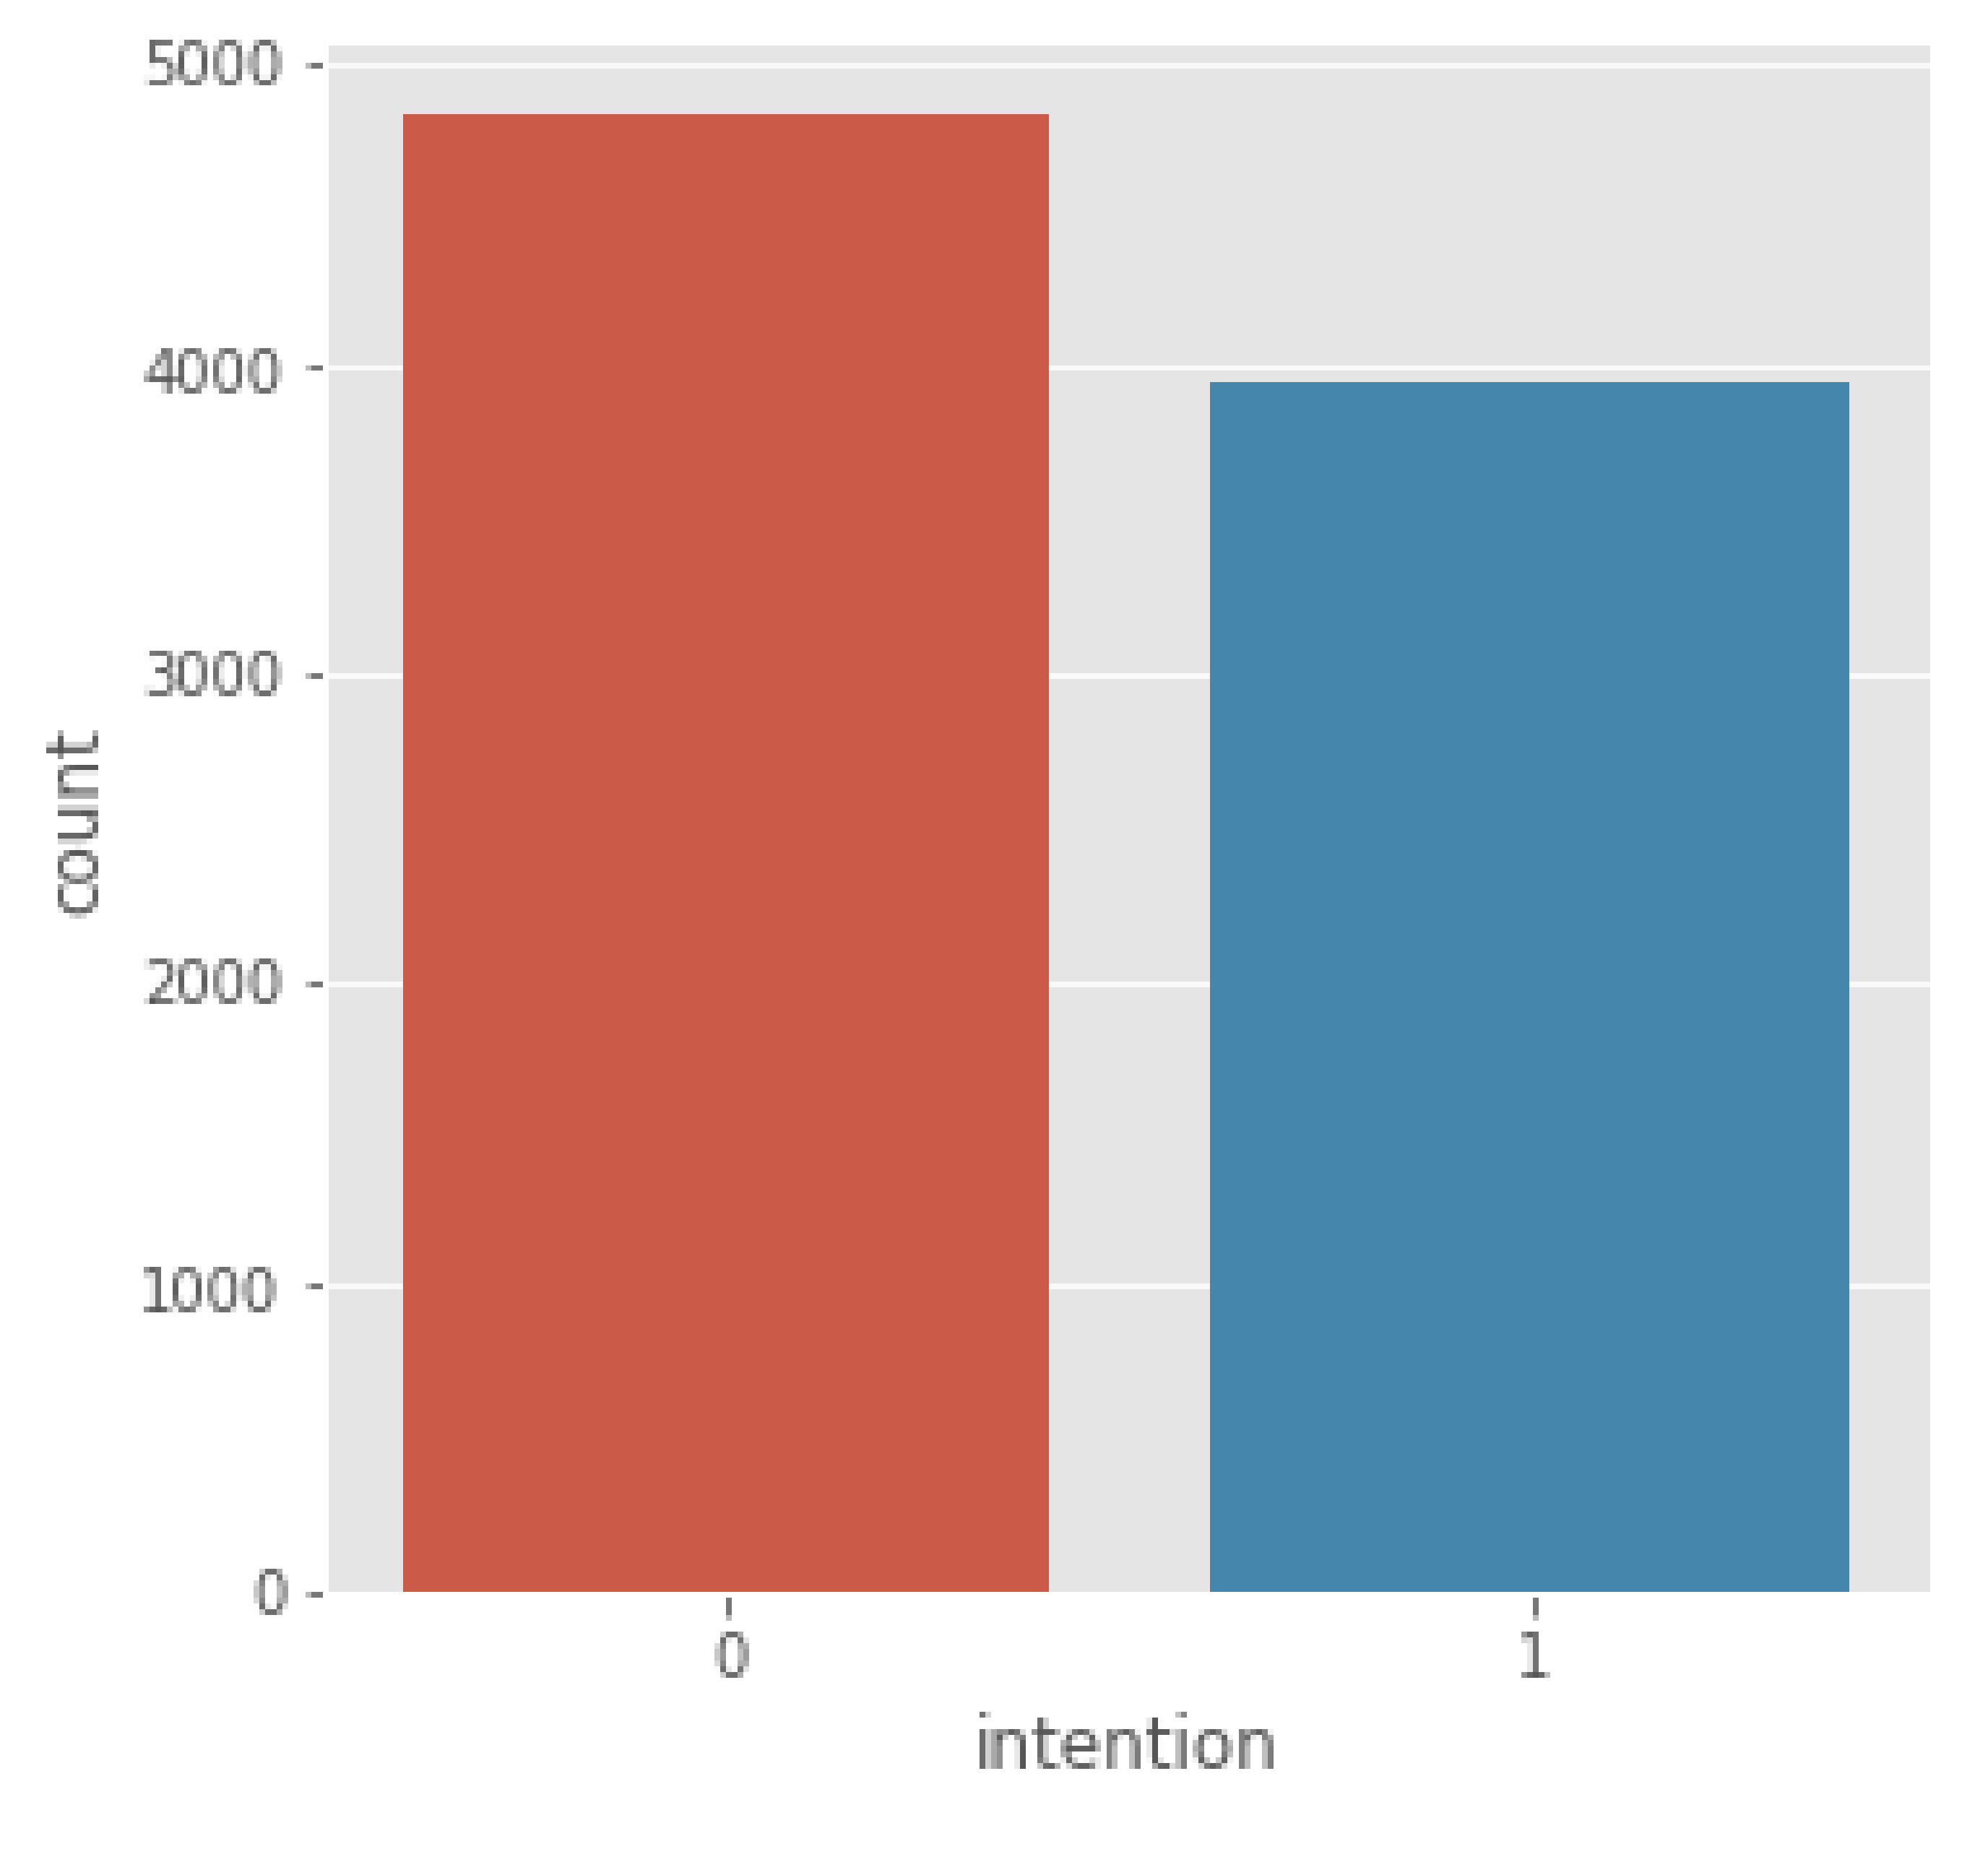
\includegraphics[width=8cm]{intentiongraph-results.png}
    \caption{Count distribution of intention after data pre-processing.} \label{fig4}
\end{figure}
\paragraph{}
In addition, the top ten word frequency and word cloud for non-suicidal and suicidal tweets are shown in \ref{table_1} and\ref{word_cloud} respectively.

\begin{figure}
\centering
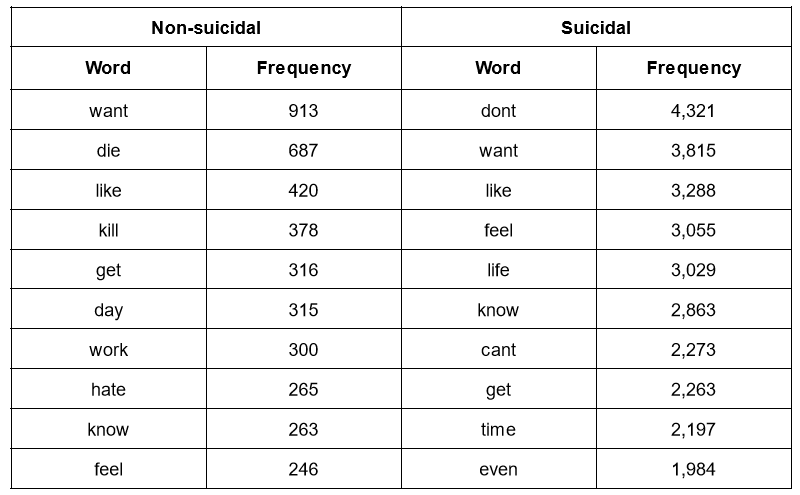
\includegraphics[width=12cm, height=8cm]{word table.png}
\captionsetup{justification=centering}
\caption{Word frequency from all non-suicidal and suicidal tweets.} \label{table_1}
\end{figure}

\paragraph \noindent Figure \ref{table_1} shows the top ten words and their respective frequency for both non-suicidal and suicidal tweets. For non-suicidal tweets, it can be seen that the top 3 words are 'want', 'die', and 'like' while in suicidal tweets the top three words are 'don't', 'want', and 'like'. It can be noticed that both 'like' and 'want' is present in non-suicidal and suicidal top 10 words. It is worth noting that words like 'die' and 'kill' are not in the top 10 words for suicidal tweets this only shows that a rigorous classification model is needed in order to accurately predict suicidal tweets from non-suicidal tweets.

\begin{figure}
  \begin{subfigure}{0.60\textwidth}
    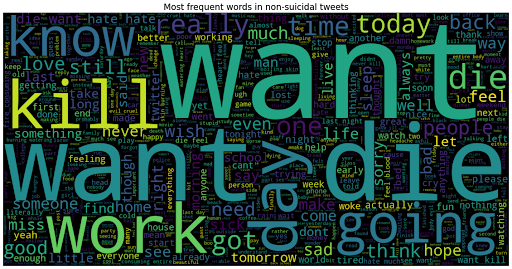
\includegraphics[width=\linewidth]{no-suicidal-intention.png}
    \caption{} \label{non-suicidal}
  \end{subfigure}%
  \hspace*{\fill}   % maximize separation between the subfigures
  \begin{subfigure}{0.60\textwidth}
    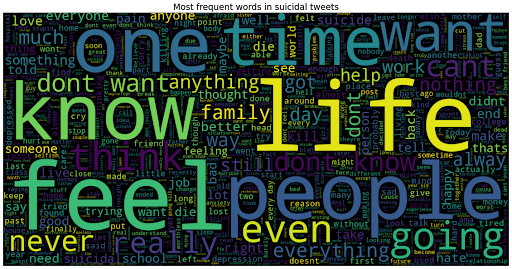
\includegraphics[width=\linewidth]{with-suicidal-intention.png}
    \caption{} \label{suicidal}
  \end{subfigure}%
  \hspace*{\fill}   % maximizeseparation between the subfigures
\captionsetup{justification=centering}
\caption{ Word Cloud for tweets with (a) non-suicidal intention and (b) suicidal intention.} \label{word_cloud}
\end{figure}

\paragraph \noindent The word cloud displays the 1000 most frequent words for the following intention categories: (a) non-suicidal and (b) with suicidal intention. The bigger words are, the more frequently the word is used. According to Joseph(2022), the commonly used ratio is 80:20, which means 80\% of the data is for training and 20\% is for testing. Other commonly used ratios are 70:30, 60:40, and 50:50. Hence, the dataset was divided into 80:20 for training and testing data, respectively.
\paragraph{}
The Twitter Suicide Intention dataset was classified using by Gaussian Naïve Bayes, Bernoulli Naïve Bayes, Random Forest, and Logistics Regression Algorithms.  

\begin{figure}
\centering
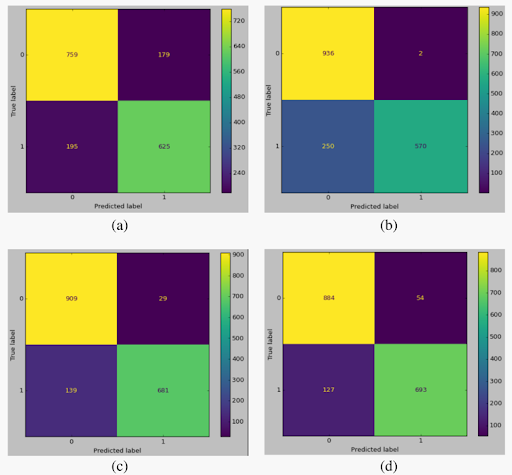
\includegraphics[width=13cm, height=8cm]{confusion.png}
\caption{Confusion matrix for GaussianNB, BernoulliNB, RandomForest and LogisticRegression} \label{confusion_matrix}
\end{figure}

\paragraph \noindent As observed in Figure \ref{confusion_matrix}, the GaussianNB classification (a) has a total of 374 mislabeled tweets, BernoulliNB (b) has 252 mislabeled tweets, RandomForest with n\_est = 400 has 168 mislabeled tweets and lastly, Logistic Regression (d) has 181 mislabeled tweets. We used the RandomForest with n\_est = 400 to represent the RandomForest classification algorithm because between the two, n\_est = 400 and n\_est = 100 the RandomForest with n\_est = 400 has fewer mislabeled tweets.

\begin{figure}
\centering
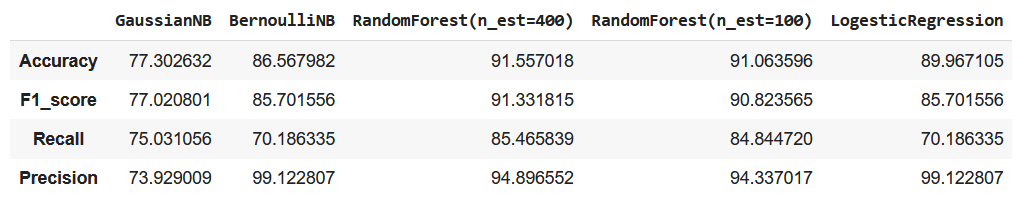
\includegraphics[width=12cm, height=2.5cm]{results.png}
\caption{Comparison table for all machine learning models used to detect suicide ideation tweets.} \label{performance_matrix}
\end{figure}

\paragraph \noindent Figure \ref{performance_matrix} shows the performance metrics of each classification models that were used. It can be observed that RandomForest with n\_est = 400 has better performance compared to other classification models. It yielded 91.557 in accuracy, 91.318 for the f1\_score, 85.4658 for recall. On the other hand, for precision the RandomForest n\_est = 400 is behind Logistic Regression and BernoulliNB which both scored 99.1228.

\paragraph \noindent Overall, the results of these classification model together with TF-IDF extraction model yielded great result in predicting suicide intentions.


\section{Conclusion}
\noindent In this study, we analyzed tweets and predicted suicidal ideation using Laxmi Kant's twitter-suicidal-intention-dataset in GitHub. We utilized the Gaussian Naive Bayes Algorithm, the Bernoulli Naive Bayes Algorithm, the Random Forest Algorithm, and the Logistics Regression Algorithm for the machine learning models.

\paragraph \noindent The experiment's findings indicated that out of all the classifiers utilized, Random Forest (n\_estimator = 400) had the most remarkable performance with an F1 measure value of 91.33\%. The experiment's findings also demonstrate that the Random Forest model with n est = 100 has a high level of accuracy, with an F1 score of 90.82\%. However, for precision the RandomForest n\_est = 400 is behind Logistic Regression and BernoulliNB.

\paragraph \noindent In addition, every other classification technique achieved a high F1 score using the feature extraction method, CountVectorizer and the TF-IDF. In conjunction with the dataset, these experiments demonstrated that utilizing CountVectorizer and TF IDF produces satisfactory results in detecting suicide ideations on twitter tweets.

\paragraph \noindent In future studies, researchers can attempt to utilize other feature extraction methods such as the ensemble and word2vec technique to assess whether or not these may improve the classification model’s performance in determining tweets with suicide intention.

% ---- Bibliography ----
%
% BibTeX users should specify bibliography style 'splncs04'.
% References will then be sorted and formatted in the correct style.
%
% \bibliographystyle{splncs04}
% \bibliography{mybibliography}
%
\begin{thebibliography}{9}
\bibitem{}
American Foundation for Suicide Prevention. (n.d.). Risk factors, protective factors, and warning signs. AFSP. Retrieved November 27, 2022, from \https://afsp.org/risk-factors-protective-factors-and-warning-signs

\bibitem{}
Chauhan, N. S. (2022, April 8). Naïve Bayes Algorithm: Everything You Need to Know. KDnuggets. Retrieved January 6, 2023, from https://www.kdnuggets.com/2020/06/naive-bayes-algorithm-everything.html

\bibitem{}
Geek Culture. (2021, August 20). How sklearn's CountVectorizer and TfidfTransformer compares with TfidfVectorizer. Medium. Retrieved January 7, 2023, from https://medium.com/geekculture/how-sklearns-countvectorizer-and-tfidftransformer-compares-with-tfidfvectorizer-a42a2d6d15a2

\bibitem{}
Geekforgeeks. (2022, November 7). Python – Lemmatization approaches with examples. https://www.geeksforgeeks.org/python-lemmatization-approaches-with-examples/

\bibitem{}
International Business Machines Corporation. (n.d.). What is Random Forest? IBM. Retrieved January 6, 2023, from https://www.ibm.com/topics/random-forest

\bibitem{}
Jessica, S. (2022, July 15). How Does Logistic Regression Work? KDnuggets. Retrieved January 6, 2023, from https://www.kdnuggets.com/2022/07/logistic-regression-work.html

\bibitem{joseph2022}
Joseph, V.  R. (2022). Optimal Ratio for Data Splitting. ResearchGate. https://www.researchgate.net/publication/358423958\_Optimal\_Ratio\_for\_Data\_Splitting

\bibitem{}
Kant, L. (2020, August 19). twitter-suicidal-intention-dataset. GitHub. Retrieved November 27, 2022, from https://github.com/laxmimerit/twitter-suicidal-intention-dataset

\bibitem{}
Kharwal, A. (2021, July 27). Bernoulli Naive Bayes in Machine Learning | Aman Kharwal. thecleverprogrammer. Retrieved January 7, 2023, from https://thecleverprogrammer.com/2021/07/27/bernoulli-naive-bayes-in-machine-learning/

\bibitem{}
Lui, J., Shi, M., \& Jang, H. (2022, July 5). Detecting Suicidal Ideation in Social Media: An Ensemble Method Based on Feature Fusion. NCBI. Retrieved November 27, 2022, from \url{https://www.ncbi.nlm.nih.gov/pmc/articles/PMC9266694/}

\bibitem{}
Luo, J., Du, J., Tao, C., Xu, H., \& Zhang, Y. (2019). Exploring temporal suicidal behavior patterns on social media: Insight from Twitter Analytics. Health Informatics Journal, 26(2), 738–752. \url{https://doi.org/10.1177/1460458219832043}

\bibitem{}
Luxton, D. D., June, J. D., \& Fairall, J. M. (2012). Social Media and suicide: A public health perspective. American Journal of Public Health, 102(S2). \url{https://doi.org/10.2105/ajph.2011.300608}

\bibitem{}
Machine Learning Library For PHP. (n.d.). Tf-idf Transformer - PHP-ML - Machine Learning library for PHP. PHP-ML. Retrieved January 7, 2023, from \url{https://php-ml.readthedocs.io/en/latest/machine-learning/feature-extraction/tf-idf-transformer/}

\bibitem{}
Martins, C. (2022, March 23). Gaussian Naive Bayes Explained and Hands-On with Scikit-Learn. Towards AI. Retrieved January 7, 2023, from \url{https://pub.towardsai.net/gaussian-naive-bayes-explained-and-hands-on-with-scikit-learn-4183b8cb0e4c}

\bibitem{}
Morese, R., Gruebner, O., Sykora, M., Elayan, S., Fadda, M., \& Albanese, E. (1AD, January 1). Detecting suicide ideation in the era of social media: The Population Neuroscience Perspective. Frontiers. Retrieved November 27, 2022, from \url{https://www.frontiersin.org/articles/10.3389/fpsyt.2022.652167/full}

\bibitem{}
O’Dea, B., Wan, S., Batterham, P. J., Calear, A. L., Paris, C., \& Christensen, H. (2015). Detecting suicidality on Twitter. Internet Interventions, 2(2), 183–188. \url{doi:10.1016/j.invent.2015.03.005}

\bibitem{}
Pianalytix. (n.d.). CountVectorizer In NLP. Pianalytix. Retrieved January 7, 2023, from \url{https://pianalytix.com/countvectorizer-in-nlp/}

\bibitem{}
Rabani, Syed \& Khan, Qamar Rayees & Khanday, Akib. (2020). Detection of Suicidal Ideation on Twitter using Machine Learning & Ensemble Approaches. Baghdad Science Journal, 17. 1328-1339. \url{10.21123/bsj.2020.17.4.1328.}

\bibitem{}
Scikit learn. (n.d.). 1.9. Naive Bayes — scikit-learn 1.1.3 documentation. Scikit-learn. Retrieved November 27, 2022, from \url{https://scikit-learn.org/stable/modules/naive\_bayes.html}

\bibitem{}
Sharma, N. (2020, June 17). Bernoulli Naive Bayes and it’s implementation | by NANDINI SHARMA. Medium. Retrieved January 7, 2023, from \url{https://medium.com/@nansha3120/bernoulli-naive-bayes-and-its-implementation-cca33ccb8d2e}

\bibitem{}
Sinyor, M., Williams, M., Zaheer, R., Loureiro, R., Pirkis, J., Heisel, M. J., Schaffer, A., Redelmeier, D. A., Cheung, A. H., & Niederkrotenthaler, T. (2020). The association between Twitter content and suicide. Australian &Amp; New Zealand Journal of Psychiatry, 55(3), 268–276. \url{https://doi.org/10.1177/0004867420969805}

\end{thebibliography}
\end{document}
